\chapter{A New Economy for An Old Problem}
\label{neweconomy}

1. In this section, I want to give a state-of-the-art of the valorisation of stubble. What is happening right now and what are the valorisation options being considered. It would be a mix of literature review with data collected from interviews and observation. 

2. Much would be estimates or explanations of how future data can complement what is known. With this part, I aim to document the state-of-the-art developments in CR and give a hint on what is senseful to work on considering the volume of PAL produced in the country.

\section{Current practices for the management of pineapple stubble}

1. Explain the cycle of the pineapple production. How it's harvested, the ratoon harvest, and then the stubble management.

2. Stubble decomposition is important because of the fly and because the sooner it's decomposed, the sooner you can plant again. Decomposition can be accelerated in many ways.

3. Explain the decomposition by agrochemicals and by fire. What you need for both and what consequences they have.

4. Explain the use of burying and its high costs and machinery use.

5. Explain the use of biodecomposers and its novelty. 

6. Summary of how all management practices have advantages and disadvantages, and how they are not ideal for the farmer because of costs, control of the fly, and management time.

\begin{comment}

\begin{figure}[H]
\caption{Structure of pineapple}
\label{pineappleStructure}
\centering
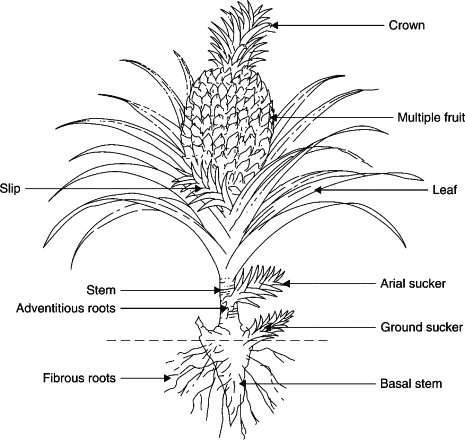
\includegraphics[width=6cm]{fig/pineappleStructure.png}

\scriptsize Source: \cite{hassan2011pineapple}
\end{figure}


The main parts of a pineapple plant are the crown, the fruit, the slips, a short and thick stem, two suckers, and a rosette of long (0.50–1.8 m), narrow, fibrous leaves. The structure of the pineapple is depicted in figure \ref{pineappleStructure}. Pineapple leaves (PAL), the biggest part of the plant, has potential to be used as a by-product for the production of many materials, or the generation of energy. Today, the PAL are not used in any valorisation process due to technological barriers and unawareness by farmers and local communities of its commercial uses \citep{jawaid2020pineapple, yusof2015novel}. 

According to a study carried out by \cite{chen2020production}, 250 tonnes of fresh pineapple plant waste are produced per hectare. The process used in their experiment demonstrated a generation of 23.3 tons of dry fibrous fibre after drying and gasification of the pulp. Considering that pineapple plantations in CR covered 40,000 harvested hectares in 2019 and that the pineapple waste is generated every two years (after the second harvest), dry fibre amounts to roughly 466,000 tonnes every year in CR. That is, for each tonne of fresh fruit produced, approximately 150 kg of dry fibre are generated. This is a relevant amount of stubble that is not only being discarded, it is also causing productivity losses to the farmers and environmental externalities to the nearby communities.

The removal and valorisation of pineapple residues after harvesting can have long-term environmental and socioeconomic advantages if value-added products can be economically produced from the pineapple residues. Pineapples leaves have commercial application potential which can add value to pineapple cultivation, facilitate extra income for entrepreneurs and farmers, and lead to agricultural diversification. 

\end{comment}

\section{Extraction from the field}

1. Extraction from the field is a big part of the puzzle to valorise the PAL. It is also a hard puzzle to solve: machinery, slope of the fields, technology that is inexistent for these conditions. 

2. Tell what has been tried (there are some things documented, other ideas are from field observation and interviews). 

3. Explain why these inventions fail from a technical point of view, and what is thought to be the solution.

4. Explain how the extraction from the field can be performed practically. Machine/workers extracting, shredding in the field itself or transporting the whole plants.

5. I gather information on costs of machinery and productivity levels (expected extraction rate, fuel/energy consumption, etc) add display on table. Again, from literature and interviews, some would be estimates.

6. Explain the (dis)advantages of using different methods and what they entail for the rest of the production of PAL-based goods (if shredding in the field then fibre is no option, for example).

\section{Potential uses of valorising pineapple stubble}

1. An in-detail description of the valorisation options being studied/implemented in CR. Stage of development and application. 

2. Costs (if available or if possible to estimate). Prices (if available or if possible to estimate). Their demand of PAL and their output estimates per tonne of PAL. 

3. A table is convenient here. It would be a good summary of the options.

\section{Demand for the potential PAL-based products}

1. Explain what is the (potential) demand of PAL-based products. I expect to give estimates based on available data online.

2. For example, for biogas, explain what can be done with it (selling to the ICE is not profitable). For fibre, there's no industry in the country. For silage, the ranchers think it makes no sense to buy it, etc.

\section{Local context and regulations applicable to PAL valorisation in CR}

1. Here I explain how regulations can affect the valorisation options.

2. Examples of what would go in this section: You cannot sell electricity privately. The bioethanol is regulated by Recope. If you want to make biobased materials to replace plastic, these must meet certain criteria, etc.


